\documentclass[tikz,border=6pt]{standalone}
\usepackage{tikz}
\usetikzlibrary{shapes,arrows,positioning,calc}
\usepackage{amsmath}

\begin{document}
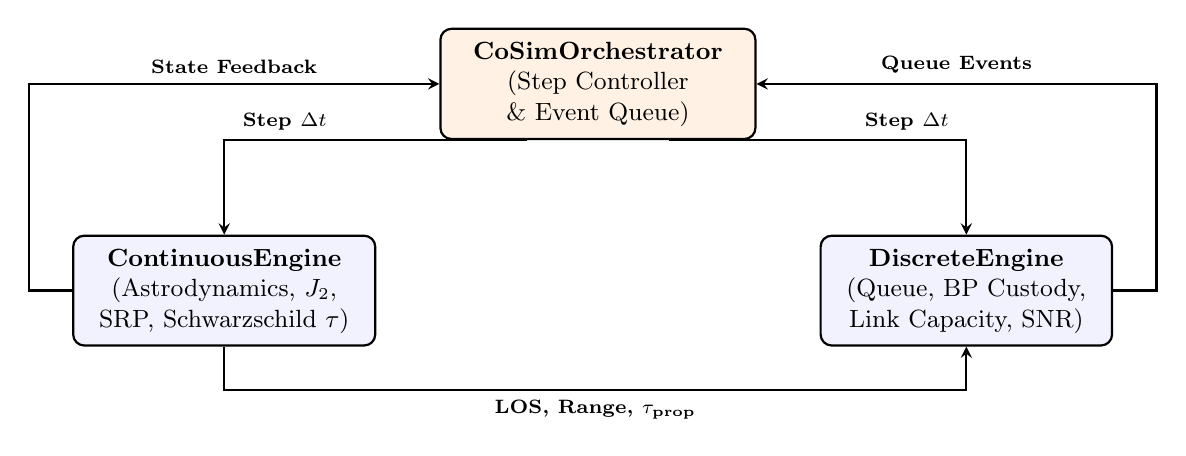
\begin{tikzpicture}[
    node distance=1.2cm and 0.8cm,
    block/.style={draw, rectangle, minimum height=1.2cm, minimum width=3.2cm,
                  align=center, rounded corners=4pt,
                  fill=blue!5, thick, font=\small},
    orch/.style={draw, rectangle, minimum height=1.4cm, minimum width=4.0cm,
                 align=center, rounded corners=4pt,
                 fill=orange!10, thick, font=\small},
    arrow/.style={thick,->,>=stealth}
]
    \node (orch) [orch] {\begin{tabular}{c}
        \textbf{CoSimOrchestrator} \\
        (Step Controller \\ \& Event Queue)
    \end{tabular}};

    \node (physics) [block, below left=of orch] {\begin{tabular}{c}
        \textbf{ContinuousEngine} \\
        (Astrodynamics, $J_2$, \\
        SRP, Schwarzschild $\tau$)
    \end{tabular}};

    \node (network) [block, below right=of orch] {\begin{tabular}{c}
        \textbf{DiscreteEngine} \\
        (Queue, BP Custody, \\
        Link Capacity, SNR)
    \end{tabular}};

    \draw [arrow] ([xshift=-0.9cm]orch.south) -|
        node[above, pos=0.4, font=\scriptsize\bfseries] {Step $\Delta t$}
        (physics.north);
    \draw [arrow] ([xshift=0.9cm]orch.south) -|
        node[above, pos=0.4, font=\scriptsize\bfseries] {Step $\Delta t$}
        (network.north);

    \draw [arrow] (physics.south) -- ++(0,-0.55) -|
        node[below, pos=0.25, font=\scriptsize\bfseries] {LOS, Range, $\tau_{\text{prop}}$}
        (network.south);
    \draw [arrow] (network.east) -- ++(0.55,0) |-
        node[above, pos=0.75, font=\scriptsize\bfseries] {Queue Events}
        (orch.east);
    \draw [arrow] (physics.west) -- ++(-0.55,0) |-
        node[above, pos=0.75, font=\scriptsize\bfseries] {State Feedback}
        (orch.west);
\end{tikzpicture}
\end{document}
